\section{Deep Gated Networks: Decoupling Neural Path Feature and Value}\label{sec:decoupled}
\begin{comment}
We encoded the gating information in the NPFs, and we saw that the decompositions of $\psi_{x,\Theta}=\psiv_{x,\Theta}+\psiv_{x,\Theta}$ and $K_{\Theta}=\kv+\kf+\kc$ captured terms related to NPF learning (and hence gating dynamics). However, from \Cref{prop:basic}, it is only known that $K_{\Theta_t}$ as a whole dictates GD dynamics. Thus, in order to ascertain that NPF learning terms $\psiv$, $\kf$ indeed make a difference, we should separate them out (from $\psi$and $K_{\Theta}$), and measure the generalisation performance with and without the NPF learning terms. This separation can be achieved by a deep gated network (see \Cref{fig:dgn} below for details) having two networks of identical architecture namely i) a feature network parameterised by $\Tg\inrdnet$, that holds gating information, and hence the NPFs and ii) a value network that holds the NPVs parameterised by $\Tv\inrdnet$.  By making $\Tg\inrdnet$ trainable/non-trainable, we can \emph{enable/disable} the NPF gradient, which gives rise to the following two modes of operating a DGN:
\end{comment}
In order to ascertain that  NPF learning indeed makes a difference, we should measure the generalisation performance with and without NPF learning. This can be achieved by a deep gated network (see \Cref{fig:dgn} below for details) having two networks of identical architecture namely i) a feature network parameterised by $\Tg\inrdnet$, that holds gating information, and hence the NPFs and ii) a value network that holds the NPVs parameterised by $\Tv\inrdnet$.  In what follows, we let $\Tdgn=(\Tg,\Tv)\in\R^{2_{dnet}}$to denote the combined parameters of a DGN. By making $\Tg\inrdnet$ trainable/non-trainable, we can \emph{enable/disable} the NPF gradient, which gives rise to the following two modes of operating a DGN:

$1.$ \textbf{Fixed NPF (FNPF):} Here, $\Tg_t=\Tg_0,\forall t\geq 0$, i.e., $\Tg\inrdnet$ is non-trainable. Thus the DGN learns the relation $\hat{y}_{\Tdgn}=\Phi^\top_{\Tg_0}v_{\Tv}$, where $\Phi_{\Tg_0}\in \R^{P\times n}$ is a fixed NPF matrix, and $v_{\Tv}$ is learned via gradient descent on $\Tv\inrdnet$.

$2.$ \textbf{Decoupled NPF Learning (DNPFL):} Here both $\Tg\inrdnet$ and $\Tv\inrdnet$ are trained, and the DGN learns the relation $\hat{y}_{\Tdgn}=\Phi^\top_{\Tg}v_{\Tv}$. In comparison to \eqref{eq:npfnpv}, here we have two parameters $\Tg\inrdnet$ and $\Tv\inrdnet$ as opposed to a single $\Theta\inrdnet$ in \eqref{eq:npfnpv}.

\textbf{Note:} FNPF and DNPFL are idealised modes to understand the role of gates, and not alternate proposals to replace standard DNNs with ReLU activations. 
\begin{figure}[h] 
\begin{minipage}{0.70\columnwidth}
\resizebox{\columnwidth}{!}{
\begin{tabular}{|l|l|l|}\hline
Layer& Feature Network (NPF)& Value Network (NPV)\\
Input & $z^{\text{F}}_{x,t}(0)=x$ &$z^{\text{V}}_{x,t}(0)=x$ \\
Activation & $q^{\text{F}}_{x,t}(l)={\Tg_t(l)}^\top z^{\text{F}}_{x,t}(l-1)$& $q^{\text{V}}_{x,t}(l)={\Tv_t(l)}^\top z^{\text{V}}_{x,t}(l-1)$\\
Hidden &$z^{\text{F}}_{x,t}(l)=\chi^{\text{F}}\left(q^{\text{F}}_{x,t}(l)\right)$& $z^{\text{V}}_{x,t}(l)=q^{\text{V}}_{x,t}(l)\odot G_{x,t}(l)$ \\
Output & None &$\hat{y}_t(x)={\Tv(d)}^\top z^{\text{V}}_{x,t}(d-1)$\\\hline
\multicolumn{3}{|l|}{Gating Values:\quad$ G_{x,t}(l)= \gamma_{r}\left(q^{\text{F}}_{x,t}(l)\right)\quad$or $G_{x,t}(l)= \gamma_{sr}\left(q^{\text{F}}_{x,t}(l)\right)$}\\\hline
\end{tabular}
}
\end{minipage}
\begin{minipage}{0.29\columnwidth}
\resizebox{\columnwidth}{!}{
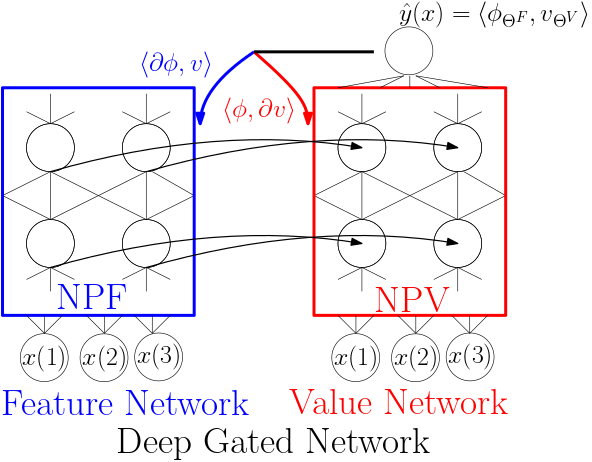
\includegraphics[scale=0.5]{figs/nntwin-blck.png}
}
\end{minipage}
\caption{Deep gated network (DGN) setup.  The pre-activations $q^{\text{F}}_{x,t}(l)$ of layer $l\in[d-1]$ from the feature network are used to derive the gating values $G_{x,t}(l)$ of layer $l\in[d-1]$. }
\label{fig:dgn}
\end{figure}
\begin{comment}
Note that, the feature network uses $\chi^{\text{F}}$ as the activation function, which can be a standard ReLU activation, i.e., $\chi^{\text{F}}=\chi_r$. The pre-activations $q^{\text{F}}_{x,t}(l)$ of layer $l\in[d-1]$ from the feature network are used to derive the gating values $G_{x,t}(l)$ of layer $l\in[d-1]$. The gating values can be obtained from either a ReLU gate $\gamma_r$ or a soft-ReLU gate $\gamma_{sr}$. The process of separating the NPFs and the NPVs decouples the value and the feature gradients. In a DGN, the value gradient $\psiv_{x,\Tdgn}$ flows through the value network and the feature gradient $\psif_{x,\Tdgn}$flows through the feature network. 
\end{comment}
\begin{proposition}[Gradient Dynamics in a DGN]\label{prop:dgn} Let $\psif_{x,\Tdgn}\stackrel{def}=\nabla_{\Tg}\hat{y}_{\Tdgn}(x) \in \R^{d_{net}}$, $\psiv_{x,\Tdgn}\stackrel{def}=\nabla_{\Tv}\hat{y}_{\Tdgn}(x) \in \R^{d_{net}}$. Let $K^{\text{V}}_{\Tdgn}$ and $K^{\text{F}}_{\Tdgn}$ be $n\times n$ matrices with entries $K^{\text{V}}_{\Tdgn}(s,s')=\ip{\psiv_{x_s,\Tdgn},\psiv_{x_{s'},\Tdgn}}$ and $K^{\text{F}}_{\Tdgn}(s,s')=\ip{\psif_{x_s,\Tdgn},\psif_{x_{s'},\Tdgn}}$. For infinitesimally small step-size of GD, the error dynamics in a DGN (in the DNPFL  and FNPF modes) is given by:
\FloatBarrier
\begin{table}[h]
\resizebox{\columnwidth}{!}{
\begin{tabular}{| l | l l l | l |}\hline
	Dynamics&		&&DNPFL& FNPF\\\hline
		&		&&& \\
Weight  & $\dot{\Theta}^{\text{V}}_t$&$=$&$-\sum_{s=1}^n \psiv_{x,\Tdgn_t}e_t(s),\dot{\Theta}^{\text{F}}_t=-\sum_{s=1}^n \psif_{x,\Tdgn_t}e_t(s)$ & $\dot{\Theta}^{\text{V}}_t$ same as (DNFPL),  $\dot{\Theta}^{\text{F}}_t=0$\\
NPF & $\dot{\phi}_{x_s,\Tg_t}(p)$&$=$&$x(\I_0(p))\sum_{\tg\in\Tg}\partial_{\tg}A_{\Tg_t}(x_s,p)\dot{\theta}^{\text{F}}_t,\forall p\in[P], s\in[n]$& $\dot{\phi}_{x_s,\Tg_t}(p)=0$\\
NPV & $\dot{v}_{\Tv_t}(p)$&$=$&$\sum_{\tv\in\Tv}\partial_{\tv}v_{\Tv_t}(p)\dot{\theta}^{\text{V}}_t,\forall p\in[P]$ & $\dot{v}_{\Tv_t}(p)$ same as DNPFL\\
%Kernel & $K_{\Tdgn}$&$=$&$K^{\text{V}}_{\Tdgn}+ K^{\text{F}}_{\Tdgn}$ & $K_{\Tdgn}=K^{\text{V}}_{\Tdgn}$ \\\hline
Error & $\dot{e}_t$&$=$&$-\left(K^{\text{V}}_{\Tdgn}+ K^{\text{F}}_{\Tdgn}\right)e_t$  & $\dot{e}_t=-\left(K^{\text{V}}_{\Tdgn}\right)e_t$ \\\hline
\end{tabular}
}
\end{table}
\end{proposition}
\textbf{Remark:} The gradient dynamics in a DGN specified in \Cref{prop:dgn} is similar to the gradient dynamics in a DNN specified in \Cref{prop:dnnhard}. Important difference is that in a DGN there are $2d_{net}$ parameters, and hence the NTF $\psi_{x,\Theta}=(\psif_{x,\Theta},\psiv_{x,\Theta})\in\R^{2d_{net}}$, wherein, $\psiv_{x,\Tdgn}\inrdnet$ flows through the value network and $\psif_{x,\Tdgn}\inrdnet$ flows through the feature network. %As a result $\kc=0$. Note that in the FNPF mode of the DGN, since $\Tg\inrdnet$ are non-trainable $\psif=0$, and hence $\dot{\phi}=0$ and $\kf=0$.